\documentclass[tikz,border=4pt]{standalone}
\usepackage[T1]{fontenc}
\usepackage[utf8]{inputenc}
\usepackage{amsmath,amssymb}
\usepackage{helvet}
\renewcommand{\familydefault}{\sfdefault}
\usepackage{pgfplots}
\pgfplotsset{compat=1.17}
\usetikzlibrary{arrows.meta,positioning,calc,fit,backgrounds,shapes.geometric}

\definecolor{cVis}{HTML}{1F77B4}
\definecolor{cTxt}{HTML}{D62728}
\definecolor{cProj}{HTML}{2CA02C}
\definecolor{cLLM}{HTML}{9467BD}
\definecolor{cConv}{HTML}{FF7F0E}
\definecolor{cAtt}{HTML}{17BECF}
\definecolor{cGray}{HTML}{7F7F7F}

\tikzset{
  blk/.style={draw, rounded corners=2pt, minimum height=8mm, align=center, font=\footnotesize, thick},
  tok/.style={draw, minimum size=3.2mm, inner sep=0pt},
  arr/.style={-{Stealth[length=2mm]}, thick},
}

\begin{document}
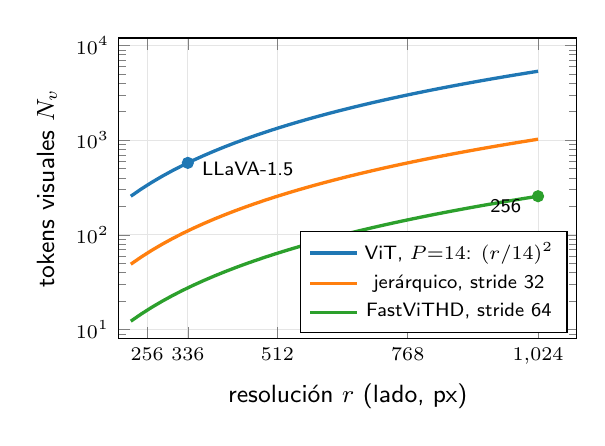
\begin{tikzpicture}
  \begin{semilogyaxis}[
    width=7.4cm, height=5.4cm, xmin=200, xmax=1100, ymin=8, ymax=12000,
    xlabel={\small resolución $r$ (lado, px)}, ylabel={\small tokens visuales $N_v$},
    xtick={256,336,512,768,1024}, xticklabel style={font=\scriptsize}, yticklabel style={font=\scriptsize},
    legend style={font=\scriptsize, at={(0.98,0.02)}, anchor=south east}, grid=major, grid style={black!10}]
    \addplot[cVis, very thick, domain=224:1024, samples=40] {(x/14)^2};
    \addlegendentry{ViT, $P{=}14$: $(r/14)^2$}
    \addplot[cConv, very thick, domain=224:1024, samples=40] {(x/32)^2};
    \addlegendentry{jerárquico, stride 32}
    \addplot[cProj, very thick, domain=224:1024, samples=40] {(x/64)^2};
    \addlegendentry{FastViTHD, stride 64}
    \addplot[only marks, mark=*, cVis] coordinates {(336,576)};
    \node[font=\scriptsize, anchor=west] at (axis cs:345,500) {LLaVA-1.5};
    \addplot[only marks, mark=*, cProj] coordinates {(1024,256)};
    \node[font=\scriptsize, anchor=east] at (axis cs:1010,200) {256};
  \end{semilogyaxis}
\end{tikzpicture}
\end{document}
